	%% ++++++++++++++++++++++++++++++++++++++++++++++++++++++++++++
%% Hauptdatei, Wurzel des Dokuments
%% ++++++++++++++++++++++++++++++++++++++++++++++++++++++++++++

% Headerfeld, Typ des Dokumentes, einzubindende Packages.
% Hier bei Bedarf Änderungen vornehmen.
\documentclass
[   twoside=false,     % Einseitiger oder zweiseitiger Druck?
    fontsize=12pt,     % Bezug: 12-Punkt Schriftgröße
    DIV=15,            % Randaufteilung, siehe Dokumentation "KOMA"-Script
    BCOR=17mm,         % Bindekorrektur: Innen 17mm Platz lassen. Copyshop-getestet.
%    headsepline,
    headsepline,  % Unter Kopfzeile Trennlinie (aus: headnosepline)
    footsepline,  % Über Fußzeile Trennlinie (aus: footnosepline)
    open=right,        % Neue Kapitel im zweiseitigen Druck rechts beginnen lassen
    paper=a4,          % Seitenformat A4
    abstract=true,     % Abstract einbinden
    listof=totoc,      % Div. Verzeichnisse ins Inhaltsverzeichnis aufnehmen
    bibliography=totoc,% Literaturverzeichnis ins Inhaltsverzeichnis aufnehmen
    titlepage,         % Titelseite aktivieren
    headinclude=true,  % Seiten-Head in die Satzspiegelberechnung mit einbeziehen
    footinclude=false, % Seiten-Foot nicht in die Satzspiegelberechnung mit einbeziehen
    numbers=noenddot   % Gliederungsnummern ohne abschließenden Punkt darstellen
]   {scrreprt}         % Dokumentenstil: "Report" aus dem KOMA-Skript-Paket

\usepackage[active]{srcltx}
\overfullrule=2cm
%\usepackage[activate=normal]{pdfcprot} % Optischer Randausgleich -> pdflatex!
\usepackage{ifthen}
\usepackage[ngerman]{babel}   % Neue Deutsche Rechtschreibung
%\usepackage[latin1]{inputenc} % Zeichencodierung nach ISO-8859-1
\usepackage[utf8]{inputenc}   %	Zeichencodierung nach UTF-8 (Unicode)
\usepackage[T1]{fontenc}
\usepackage{graphicx}
%\usepackage{ae} % obsolet und durch lmodern ersetzt
\usepackage{lmodern}
\usepackage{listings}
\usepackage[T1]{url}
\usepackage{amsthm}
\usepackage{amsmath}
\usepackage{graphicx}
\RequirePackage{scrlfile}
\ReplacePackage{scrpage2}{scrlayer-scrpage}
% old: \usepackage[automark]{scrpage2}
\usepackage[automark]{scrlayer-scrpage}
\usepackage{setspace}
%\usepackage[first,light]{draftcopy} % Für Probedruck
\usepackage[plainpages=false,pdfpagelabels,hypertexnames=false]{hyperref}



%% UNIX 
\makeatletter
\DeclareOldFontCommand{\rm}{\normalfont\rmfamily}{\mathrm}
\DeclareOldFontCommand{\sf}{\normalfont\sffamily}{\mathsf}
\DeclareOldFontCommand{\tt}{\normalfont\ttfamily}{\mathtt}
\DeclareOldFontCommand{\bf}{\normalfont\bfseries}{\mathbf}
\DeclareOldFontCommand{\it}{\normalfont\itshape}{\mathit}
\DeclareOldFontCommand{\sl}{\normalfont\slshape}{\@nomath\sl}
\DeclareOldFontCommand{\sc}{\normalfont\scshape}{\@nomath\sc}
\makeatother

%% 

% Tiefe der Kapitelnummerierung beeinflussen
\setcounter{secnumdepth}{3} % Tiefe der Nummerierung
\setcounter{tocdepth}{3}    % Tiefe des Inhaltsverzeichnisses

% Datum anpassen
\newcommand{\leadingzero}[1]{\ifnum #1<10 0\the#1\else\the#1\fi}
\renewcommand{\today}{\leadingzero{\day}.\leadingzero{\month}.\the\year}     % DD.MM.YYYY

% Hier in die zweite geschweifte Klammer jeweils
% die persoenlichen Daten und das Thema der Arbeit eintragen:
\newcommand{\artderausarbeitung}{Reviewdokument zur Implementierungsphase}
\newcommand{\namedesautorsI}{P.~Augustin, J.~Skopp, C.~Juin, }
\newcommand{\namedesautorsII}{G.~Lehmann, A.~Schmidt, R.~Schöne}
\newcommand{\themaderarbeit}{RION Package-Manager}
\newcommand{\xRION}{\RION}
%% Das passt schon so 
\newcommand{\namedesautors}{\namedesautorsI \namedesautorsII}

% PDF Metadaten definieren
\hypersetup{
   pdftitle={\themaderarbeit},
   pdfsubject={\artderausarbeitung},
   pdfauthor={\namedesautors},
   pdfkeywords={\artderausarbeitung; TU-Ilmenau}}


% Abkürzungsverzeichnis beeinflussen. Hier nichts ändern!
\usepackage[intoc]{nomencl}
  \AtBeginDocument{\setlength{\nomlabelwidth}{.25\columnwidth}}
  \let\abbrev\nomenclature
  \renewcommand{\nomname}{Abkürzungsverzeichnis und Formelzeichen}
  \renewcommand{\nomlabel}[1]{#1 \dotfill}
  \setlength{\nomitemsep}{-\parsep}
  \makenomenclature

\usepackage[normalem]{ulem}
  \newcommand{\markup}[1]{\textbf{#1}}

% Seitenlayout festlegen. Hier nichts ändern!
\pagestyle{scrplain}
\ihead[]{\headmark}
\ohead[]{\pagemark}
\chead[]{}
\ifoot[]{}
\ofoot[]{\scriptsize \artderausarbeitung\ - \namedesautors}
\cfoot[]{}
\renewcommand{\titlepagestyle}{scrheadings}
\renewcommand{\partpagestyle}{scrheadings}
\renewcommand{\chapterpagestyle}{scrheadings}
\renewcommand{\indexpagestyle}{scrheadings}



% Abschnittsweise Nummerierung anstatt fortlaufend. Hier nichts ändern!
\makeatletter
\@addtoreset{equation}{chapter}
\@addtoreset{figure}{chapter}
\@addtoreset{table}{chapter}
\renewcommand\theequation{\thechapter.\@arabic\c@equation}
\renewcommand\thefigure{\thechapter.\@arabic\c@figure}
\renewcommand\thetable{\thechapter.\@arabic\c@table}
\makeatother
\renewcommand*{\pagedeclaration}[1]{\unskip, \hyperpage{#1}}

% Quelltextrahmen, klein. Hier nichts ändern!
\newsavebox{\inhaltkl}
\def\rahmenkl{\sbox{\inhaltkl}\bgroup\small\renewcommand{\baselinestretch}{1}\vbox\bgroup\hsize\textwidth}
\def\endrahmenkl{\par\vskip-\lastskip\egroup\egroup\fboxsep3mm%
\framebox[\textwidth][l]{\usebox{\inhaltkl}}}

% Quelltextrahmen, normale Groesse. Hier nichts ändern!
\newsavebox{\inhalt}
\def\rahmen{\sbox{\inhalt}\bgroup\renewcommand{\baselinestretch}{1}\vbox\bgroup\hsize\textwidth}
\def\endrahmen{\par\vskip-\lastskip\egroup\egroup\fboxsep3mm%
\framebox[\textwidth][l]{\usebox{\inhalt}}}


% Sonstige Befehlsdefinitionen hier ablegen.
\newcommand{\entspricht}{\stackrel{\wedge}{=}}
\newcommand{\quotes}[1]{\glqq#1\grqq{}}
\newcommand{\x}{X-FAB} % sry :)
\newcommand{\e}{RION} % well
\newcommand{\Linux}{GNU/Linux}
\makenomenclature


% Tabellenspaltendefinitionen mit fester Breite --> somit Zeilenumbruch innerhalb einer Zelle möglich
% aus http://www.torsten-schuetze.de/tex/tabsatz-2004.pdf
\usepackage{array, booktabs}
\newcolumntype{f}{>{$}l<{$}}
\newcolumntype{n}{>{\raggedright}l}
\newcolumntype{N}{>{\scriptsize}l}
\newcolumntype{v}[1]{>{\raggedright\hspace{0pt}}m{#1}}
\newcolumntype{V}[1]{>{\scriptsize\raggedright\hspace{0pt}}m{#1}}
\newcolumntype{Z}[1]{>{\raggedright\centering}m{#1}}
\newcolumntype{k}[1]{>{\raggedright}p{#1}}
% ergibt Tabllenspalte fester Breite, linksbündig
% Umbruch innerhalb der Zelle mit \\, neue Tabellezeile mit \tabularnewline
% \addlinespace für Gruppentrennung (aus \texttt{booktabs.sty})


\begin{document}
\onehalfspacing

\begin{titlepage}
	\centering
	{\Large \textsc{Technische Universität Ilmenau}}\\[3ex]
	{\Large Rechnerarchitekturen und Eingebettete Systeme}\\[3ex]
	\vfill
	{\Large \textbf{\artderausarbeitung}}\\[4ex]
	{\large \textbf{\themaderarbeit}}\\[5ex]
	%{\large \textbf{\xRION}}\\[5ex]
	\vfill
	\begin{tabular}{rl}
		\hline\\
		vorgelegt von:          & \quad \namedesautorsI\\[1,5ex]
										       & \quad \namedesautorsII\\[1,5ex]
		eingereicht am:         & \quad 
		\today \\[1,5ex]
		Fachgebiet:            & \quad Rechnerarchitekturen und Eingebettete Systeme\\[0,5ex]
								& \quad Institut für Mikroelektronik- und Mechatronik-System\\[1,5ex]
		Betreuer:            	& \quad Georg Gläser, Andreas Becher \\[1,5ex]
		Seminarleiter           & \quad Prof. Armin Zimmermann \\[1,5ex]	
	\end{tabular}
	\vfill
	
    


\end{titlepage}
%%% ++++++++++++++++++++++++++++++++++++++++++++++++++++++++++++
%% Zusammenfassung, Abstract
%% ++++++++++++++++++++++++++++++++++++++++++++++++++++++++++++


\renewcommand{\abstractname}{Kurzfassung}
\begin{abstract}
	\begin{center}
		X-FAB bietet eine Fülle an unterschiedlichen Technologien für diverse und auch
        spezifische Anwendungsmärkte an. Um Packete für das Process Design Kit verwalten zu können soll ein Package-Manager mit dem Namen RION geschaffen werden
	\end{center}
\end{abstract}

% Inhaltsverzeichnis
\cleardoublepage % Seitenumbruch erzwingen vor Änderung des Nummerierungsstils
\pagenumbering{roman} % Nummerierung der Seiten ab hier: i, ii, iii, iv...
\pagestyle{scrheadings} % Ab hier mit Kopf- und Fusszeile
\tableofcontents

% Die einzelnen Kapitel
\cleardoublepage % Seitenumbruch erzwingen vor Änderung des Nummerierungsstils
\pagenumbering{arabic} % Nummerierung der Seiten ab hier: 1, 2, 3, 4...

%%% Content %%%
\part*{Review Documentation}

\chapter{Einleitung}
\section{Zweck des Systems}
Aufgabe ist die Erstellung eines Packagemanagers zur Suche, Installation, Aktualisierung
und Verwaltung von PDKs. 

\section{Entwurfsziele}
Der Packagemanager sollte in Python geschrieben werden.\\

Zuzüglich der oben genannten Ziele, sollte der Packagemanager auch das Management von
Abhängigkeiten, das Verwalten von virtuellen Umgebungen, sowie das Erkennen von bereits
installierten Paketen ermöglichen. Zudem sollten auch zu jedem Paket ein Informationstext
in Form von bereits vorliegenden Textdateien angezeigt werden können.\\


Serverseitig soll ein Programm die verfügbaren Pakete verwalten können. In einer
Datenbank, sollen der Name des Paketes, noch festzulegende Metadaten und
Abhängigkeiten gespeichert sein. Außerdem sollte der Server natürlich, dem
Packagemanager die Pakete selbst bereit stellen. \\

Client und Server zusammen sollen desweiteren über eine Rechteverwaltung bzw.
Authentifizierung verfügen, welche es verschieden Nutzern ermöglicht auf verschiedene
Pakete zuzugreifen.

\clearpage
\section{Überblick}
Implementiert wurden zum jetzigen Stand folgende Punkte:


\begin{itemize}
    \item  Entfernen von Paketen
    \item Suchen von Paketen
    \item Nutzerauthentifizierung
    \item Übertragung von Paketen vom Server zum Client
   \item Verwalten von virtuellen Umgebungen
   \item Installation von Paketen
 \item Konfigurationdatei
\end{itemize}

Noch nicht Implementiert sind:
\begin{itemize}
    \item Abhängigkeitenverwaltung
     \item Programm zur Verwaltung der auf dem Server verfügbaren Paketen
\end{itemize}
\chapter{Grobentwurf}
\\[\intextsep]
\begin{minipage}{\linewidth}
\centering%
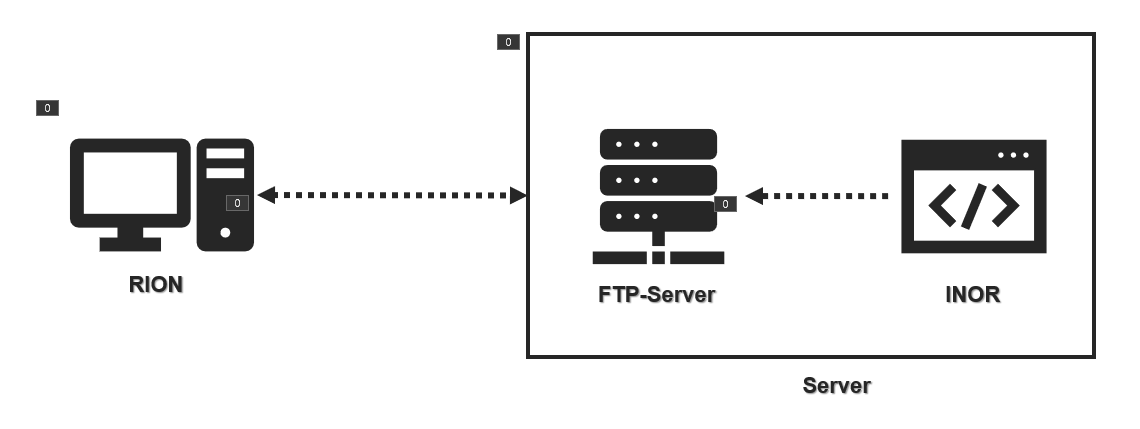
\includegraphics[width=0.8\linewidth,clip=]{./img/Img1.jpg}%
\label{fig:Image 1}%
\end{minipage}
\\[\intextsep]

Das Programm arbeitet prinzipiell mit drei Komponenten. Zum einen gibt es den
Packagemanger RION. Dieser läuft auf dem jeweiligen Endgerät (Client), der Pakete sucht,
installiert, aktualisiert, entfernt und verwaltet. Hierzu werden mehrere Datenbanken
verwendet. Darunter eine Datenbank, die eine Liste aller installierten Pakete enthält und eine
Andere, mit einer Liste der Namen aller verfügbaren Pakete, sowie deren Metadaten und die
Namen der notwendigen Abhängigkeiten. \\


Die Pakete sowie die zweite genannte Datenbank können von einem FTP-Server über eine
verschlüsselte ftps-Verbindung abgerufen werden. Hierzu wird das Programm pyftpdlib,
welches unter anderem virtuelle Nutzer zur Verfügung stellt, die zum Rechtemanagement
verwendet werden. (Dieses Programm wird nicht nicht von uns entwickelt.)
\\

Die Daten für den FTP-Server sowie die Konfiguration der Rechteverwaltung werden durch
die Dritte Komponente INOR zur Verfügung gestellt. Welche diesen Vorgang durch einige
Funktionen erleichtert bzw. automatisiert. INOR befindet sich dabei auf dem selben Server,
wie der FTP-Server.\\   
\chapter{Realisierter Entwurf}
\section{altes Klassendiagramm}
[\intextsep]
\begin{minipage}{\linewidth}
\centering%
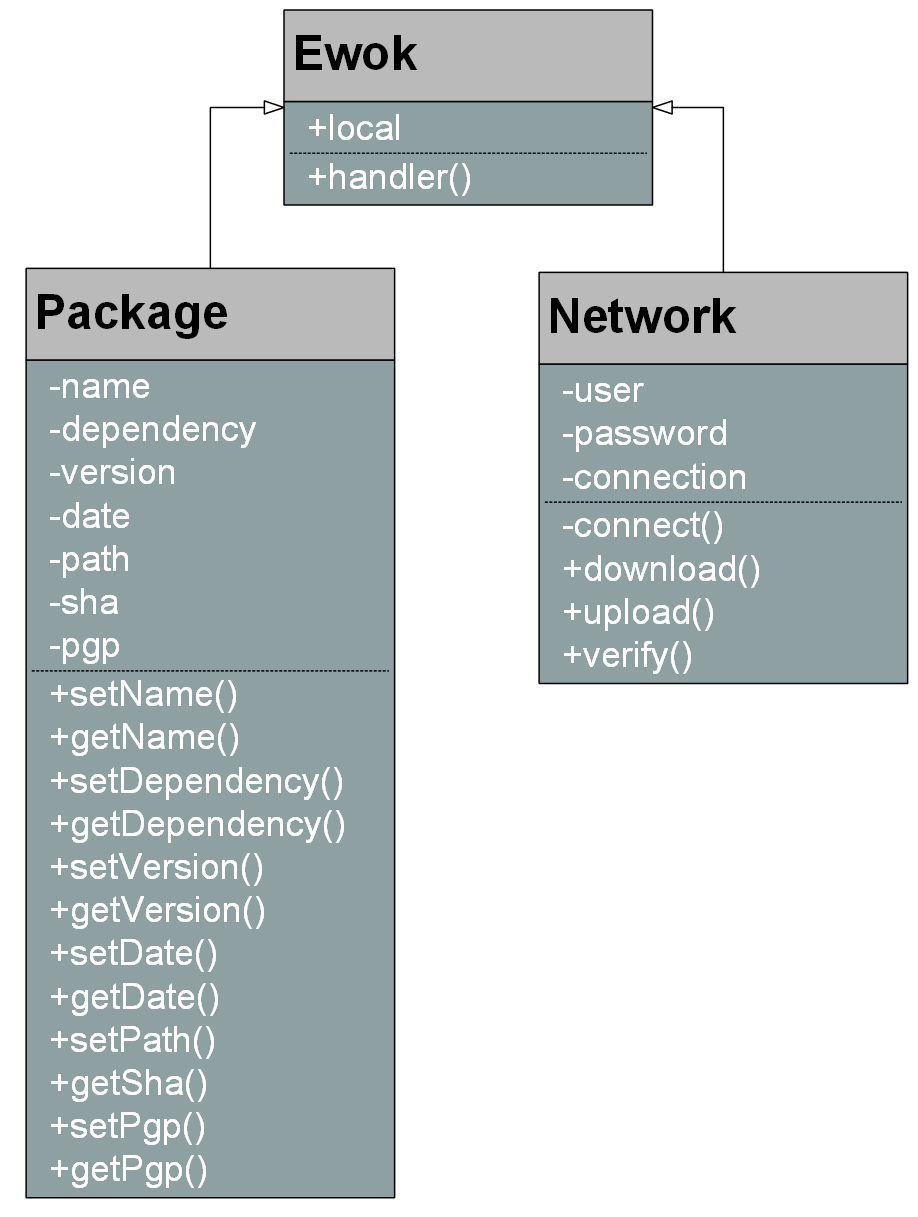
\includegraphics[width=0.8\linewidth,clip=]{./img/Img2.jpg}%
\label{fig:altes_Klassendiagramm}%
\end{minipage}
[\intextsep]


\section{neues Klassendiagramm}
[\intextsep]
\begin{minipage}{\linewidth}
\centering%
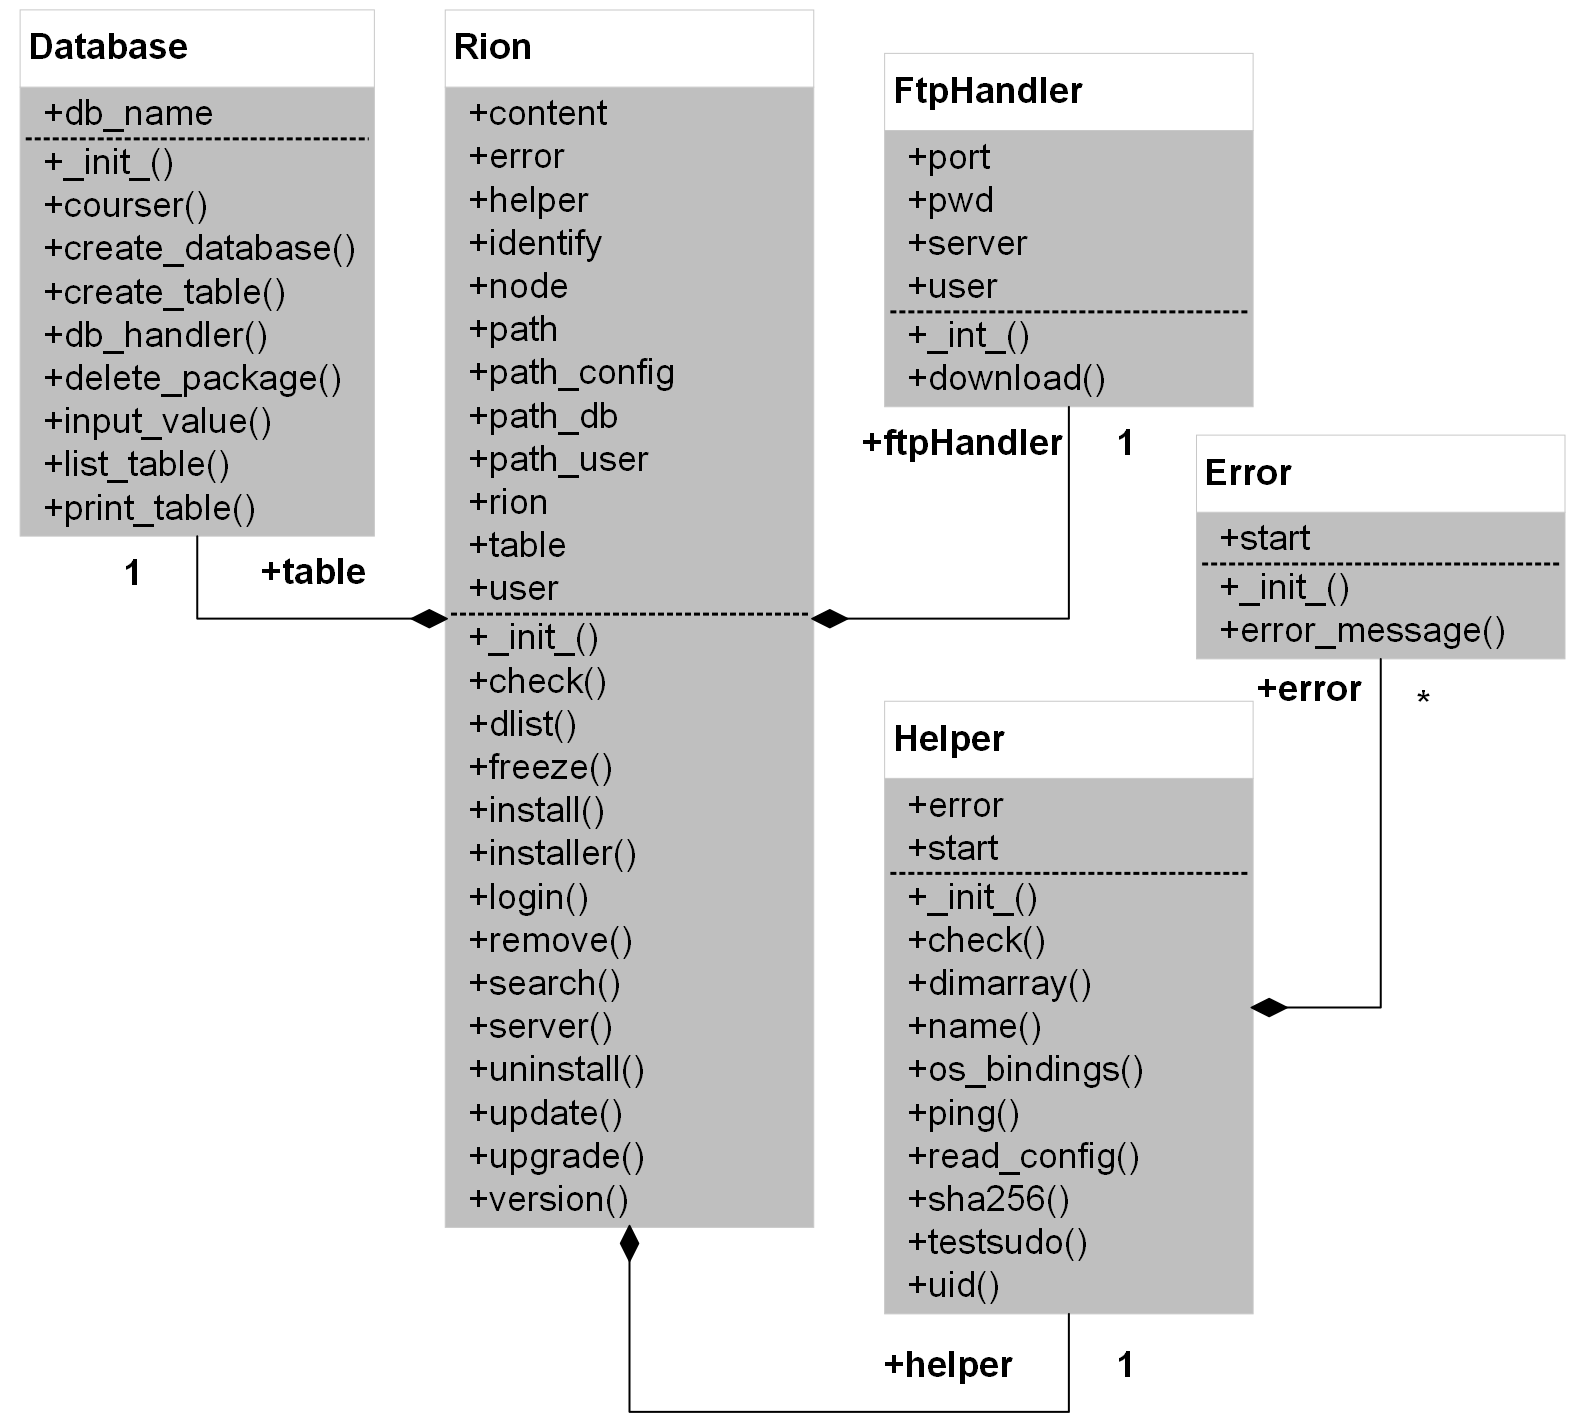
\includegraphics[width=0.8\linewidth,clip=]{./img/Img3.jpg}%
\label{fig:altes_Klassendiagramm}%
\end{minipage}
[\intextsep]

In der Implementierungsphase wurde die Erstellung eines neuen Klassendiagramms, aufgrund von Unzulänglichkeiten des vorigen, notwendig.
    
    
\section{Sequenzdiagramm}
[\intextsep]
\begin{minipage}{\linewidth}
\centering%
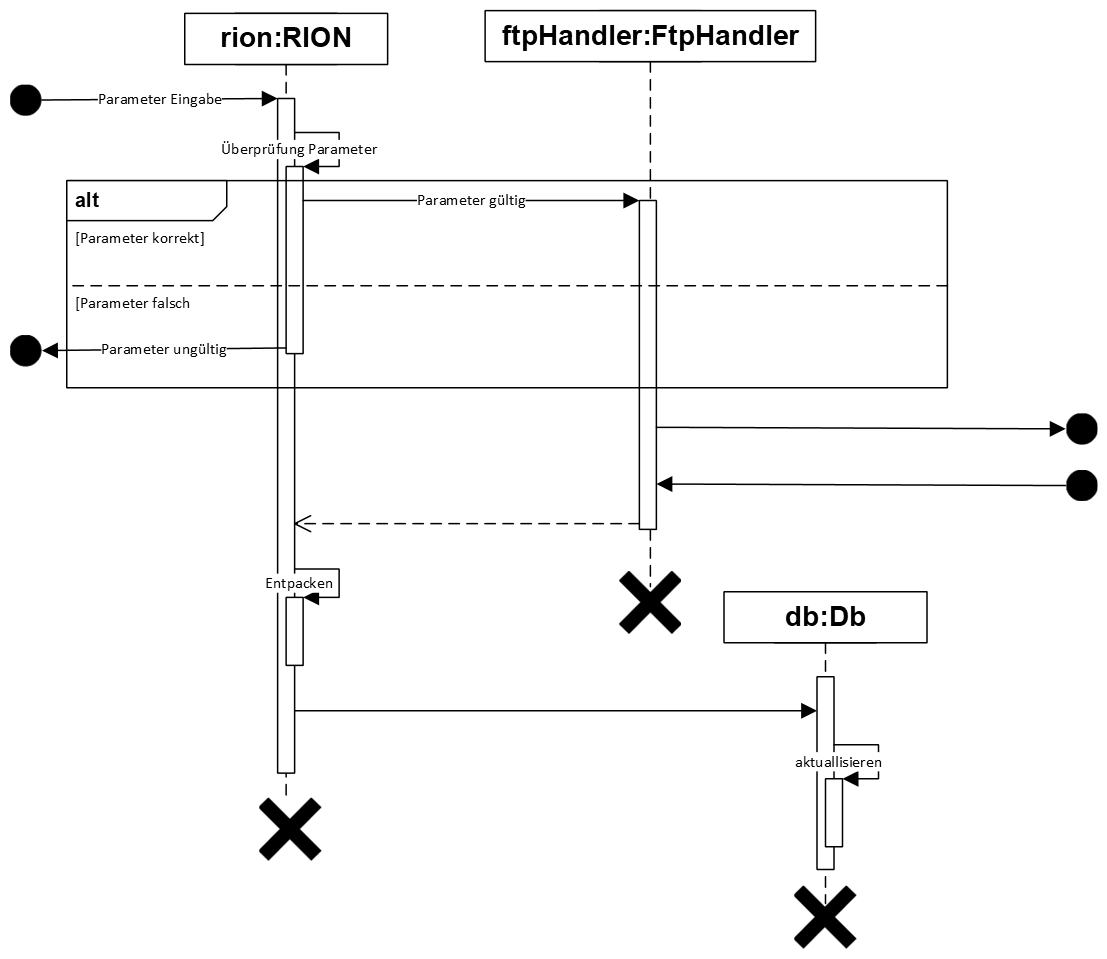
\includegraphics[width=0.8\linewidth,clip=]{./img/Img4.jpg}%
\label{fig:altes_Klassendiagramm}%
\end{minipage}
[\intextsep]
\clearpage

Entscheidung 1\\
Aufgabe: Protokoll, mit dem RION auf die Pakete des Servers zugreift\\

Ursprünglich war geplant, RION und INOR via Client-Server-Modell eng miteinader zu
verbinden. In der eigentlichen Implemetierung stellte sich jedoch heraus, dass ein
klassischer Ansatz sinnvoller ist. \\

Inor arbeitet unabhängig von RION. Seine Aufgabe besteht allein darin, Ordner mit Paketen
bzw. physischen Links auf Pakete zu befüllen. Auf diese wird dann mittels eines Protokolls
zugegriffen. Hierfür gibt es primär zwei verschlüsselte Optionen:\\

\begin{itemize}
    \item Option 1: https
    \begin{itemize}
        \item Vorteile:
            \begin{itemize}
                \item beste Übertragungsgeschwindigkeit
            \end{itemize}
        \item Nachteile:
            \begin{itemize}
                \item Arbeitet nicht direkt auf Dateienebene
                \item Aufwendige Implementierung der Authentifikation
            \end{itemize}
    \end{itemize}
     \item Option 2: ftps
    \begin{itemize}
        \item Vorteile
        \begin{itemize}
        \item Arbeitet direkt auf der Dateienebene
        \item pyftpflib bietet bereits eine ausgereifte und gut getestete Implemtierung zur
Authentifikation in Form von virtuellen Nutzern
        \end{itemize}
        \item Nachteile
        \begin{itemize}
            \item Nicht die beste, aber immer noch eine sehr gute Geschwindigkeit
        \end{itemize}
        Konklusion: Aufgrund der Möglichkeit virtuelle Nutzer anzulegen, ist ftps aus unserer Sicht
die für RION/INOR richtige Entscheidung.


        
    \end{itemize}
\end{itemize}
\clearpage

Entscheidung 2 \\
Aufgabe: Festlegen eines Tools zur Verwaltung von installierbaren und installierten Paketen.

\begin{itemize}
    \item Option 1: Sqlite3
    \begin{itemize}
        \item Vorteile
        \begin{itemize}
            \item native Einbindung
            \item komplexe Anfragen funktionieren einfacher
            \item leichtgewichtig
        \end{itemize}
        \item Nachteile
                
        \begin{itemize}
            \item Nicht ohne entsprechendes Programm lesbar
            \item Entsprechende Binarys für jede Plattform
        \end{itemize}
    \end{itemize}
     \item Option 2: json  
    \begin{itemize}
        \item Vorteile
        \begin{itemize}
            \item leichtgewichtiger
            \item plain text
        \end{itemize}
        \item Nachteile
        \begin{itemize}
            \item unübersichtlich bei großen Datenmengen
        \end{itemize}        
    \end{itemize}
\end{itemize}

Konklusion: Sqlite3 mag den Nachteil haben, dass es normalerweise eine systemspezifische
Binary benötigt, das wird jedoch durch die Einbindung in Python umgangen. Dies, kombiniert
mit den einfachen Möglichkeiten für komplexe Anfragen, hat den Ausschlag für Sqlite3
gegeben.

    
% This file is a ghost. Only abbreviations for foreign words or new words are stored here. Nothing more
\makenomenclature
\nomenclature{RION}{Packagemanager und Schnittstelle für die Paketverwaltung zwischen X-FAB-Server und Client}

\nomenclature{X-FAB}{Die X-FAB ist ein Anbieter für Halbleitertechnologien, welcher sowohl die Fertigung als auch Designunterstützung für Kunden anbietet, die gemischt analog-digitale integrierte Schaltkreise (ICs) entwickeln. Die X-FAB bietet eine Reihe an unterschiedlichen Technologien für diverse und auch
spezifische Anwendungsmärkte an.}

\nomenclature{INOR}{Serverseitiges BackEnd bei der X-FAB.}

\nomenclature{Pakete/Packages}{Datenbündel, die als solches eine Funktion haben. Hiermit sind die Pakete auf den X-FAB-Servern gemeint.}

\nomenclature{pyftpdlib}{FTP-Server-Implementation für Python}

\nomenclature{Python}{Programmiersprache: \url{https://www.python.org/}}

\nomenclature{CLI}{Ein \texttt{C}ommand \texttt{L}ine \texttt{I}nterface ist eine Schnittstelle, die es dem Nutzer erlaubt, Textbefehle an ein Programm zu übermitteln. Betriebssysteme, darunter GNU/Linux stellen hierfür eine sogenannte Shell, wie zum Beispiel Bash, Dash oder ZSH, zur Verfügung, auf welche man mit einem Terminal zugreifen kann.}

\nomenclature{Manpage}{Eine Hilfeseite für installierte Programme unter Unix-artigen Systemen, auf der für gewöhnlich Befehle, Flags und Hinweise zur Benutzung eines Programms verzeichnet sind. Darauf zugegriffen wird mit \texttt{man >>name<<}.}

\nomenclature{pip}{Python Package-Manager: \url{https://pypi.org/project/pip/}}

\nomenclature{PDK}{Ein PDK ist eine komplexe Sammlung von technologiespezifischen Daten für den aufwändigen und
relativ teuren Entwurf von anwendungsspezifischen integrierten Schaltkreisen.}

\nomenclature{PyPi}{Pypi ist eine Softwaresammlung, durch die Pythonpackages via pip heruntergeladen werden können.}

\printnomenclature
%%% Ende %%%

%\appendix
%\part*{Anhang}


% Anahng
%%% ++++++++++++++++++++++++++++++++++++++++++++++++++++++++++++
%% Anhang: Literaturverzeichnis
%% ++++++++++++++++++++++++++++++++++++++++++++++++++++++++++++


% Mit dem Befehl \nocite werden auch nicht im Text zitierte
% aus der Literaturdatenbank mit in das Literaturverzeichnis aufgenommen.
% Ein "\nocite{*}" übernimmt ungeprüft die komplette Datenbank.
%\nocite{*}

\cleardoublepage
\nocite{*}
\ihead[]{Literaturverzeichnis}
\bibliographystyle{acm}
\bibliography{literatur} % "literatur.bib" ist hier die einzige Literaturdatenbank.

% Alternativ: Mehrere Datenbanken verwenden, falls eine
% oder mehrere umfangreiche Sammlungen exisitieren:
%\bibliography{literatur_buecher,literatur_weblinks}


%% ++++++++++++++++++++++++++++++++++++++++++++++++++++++++++++
%% Anhang: Abbildungsverzeichnis
%% ++++++++++++++++++++++++++++++++++++++++++++++++++++++++++++


% Keine Änderungen vornehmen!
\cleardoublepage
\ihead[]{Abbildungsverzeichnis}
\listoffigures


%% ++++++++++++++++++++++++++++++++++++++++++++++++++++++++++++
%% Anhang: Abkürzungsverzeichnis
%% ++++++++++++++++++++++++++++++++++++++++++++++++++++++++++++


% Hier keine weiteren Änderungen vornehmen
\cleardoublepage
\ihead[]{Abkürzungsverzeichnis und Formelzeichen}
\printnomenclature{} % TODO: Hyperref




\end{document}
